\documentclass{standalone}
\author{Quinten Bruynseraede}
\usepackage{tikz}
\usetikzlibrary{shapes}
\title{Tikz grafen}
\begin{document}\pagestyle{empty}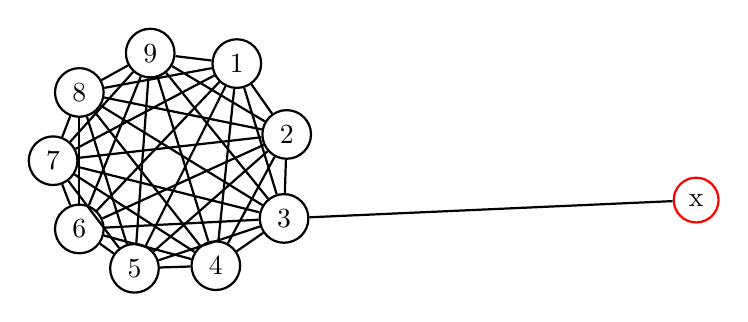
\begin{tikzpicture}\node[shape=circle,draw=black,align=center,line width=0.8pt] (0) at (0.7,9.033333333333333) {7};
\node[shape=circle,draw=black,align=center,line width=0.8pt] (1) at (1.0333333333333334,9.9) {8};
\node[shape=circle,draw=black,align=center,line width=0.8pt] (2) at (1.9333333333333333,10.4) {9};
\node[shape=circle,draw=black,align=center,line width=0.8pt] (3) at (3.033333333333333,10.266666666666667) {1};
\node[shape=circle,draw=black,align=center,line width=0.8pt] (4) at (3.6666666666666665,9.366666666666667) {2};
\node[shape=circle,draw=black,align=center,line width=0.8pt] (5) at (3.6333333333333333,8.3) {3};
\node[shape=circle,draw=black,align=center,line width=0.8pt] (6) at (2.7666666666666666,7.7) {4};
\node[shape=circle,draw=black,align=center,line width=0.8pt] (7) at (1.7333333333333334,7.666666666666667) {5};
\node[shape=circle,draw=black,align=center,line width=0.8pt] (8) at (1.0333333333333334,8.166666666666666) {6};
\node[shape=circle,draw=red,align=center,line width=0.8pt] (9) at (8.866666666666667,8.533333333333333) {x};

\path [-,draw=black,line width=0.8pt] (2) edge node {} (3);
\path [-,draw=black,line width=0.8pt] (3) edge node {} (4);
\path [-,draw=black,line width=0.8pt] (4) edge node {} (5);
\path [-,draw=black,line width=0.8pt] (5) edge node {} (6);
\path [-,draw=black,line width=0.8pt] (6) edge node {} (7);
\path [-,draw=black,line width=0.8pt] (7) edge node {} (8);
\path [-,draw=black,line width=0.8pt] (8) edge node {} (0);
\path [-,draw=black,line width=0.8pt] (0) edge node {} (1);
\path [-,draw=black,line width=0.8pt] (1) edge node {} (2);
\path [-,draw=black,line width=0.8pt] (2) edge node {} (4);
\path [-,draw=black,line width=0.8pt] (2) edge node {} (5);
\path [-,draw=black,line width=0.8pt] (2) edge node {} (6);
\path [-,draw=black,line width=0.8pt] (2) edge node {} (7);
\path [-,draw=black,line width=0.8pt] (2) edge node {} (8);
\path [-,draw=black,line width=0.8pt] (2) edge node {} (0);
\path [-,draw=black,line width=0.8pt] (3) edge node {} (1);
\path [-,draw=black,line width=0.8pt] (3) edge node {} (0);
\path [-,draw=black,line width=0.8pt] (3) edge node {} (8);
\path [-,draw=black,line width=0.8pt] (3) edge node {} (7);
\path [-,draw=black,line width=0.8pt] (3) edge node {} (6);
\path [-,draw=black,line width=0.8pt] (3) edge node {} (5);
\path [-,draw=black,line width=0.8pt] (4) edge node {} (1);
\path [-,draw=black,line width=0.8pt] (4) edge node {} (0);
\path [-,draw=black,line width=0.8pt] (4) edge node {} (8);
\path [-,draw=black,line width=0.8pt] (4) edge node {} (7);
\path [-,draw=black,line width=0.8pt] (4) edge node {} (6);
\path [-,draw=black,line width=0.8pt] (5) edge node {} (1);
\path [-,draw=black,line width=0.8pt] (5) edge node {} (0);
\path [-,draw=black,line width=0.8pt] (5) edge node {} (8);
\path [-,draw=black,line width=0.8pt] (5) edge node {} (7);
\path [-,draw=black,line width=0.8pt] (6) edge node {} (1);
\path [-,draw=black,line width=0.8pt] (6) edge node {} (0);
\path [-,draw=black,line width=0.8pt] (6) edge node {} (8);
\path [-,draw=black,line width=0.8pt] (7) edge node {} (1);
\path [-,draw=black,line width=0.8pt] (7) edge node {} (0);
\path [-,draw=black,line width=0.8pt] (8) edge node {} (1);
\path [-,draw=black,line width=0.8pt] (5) edge node {} (9);
\end{tikzpicture}
\end{document}